\begin{center}
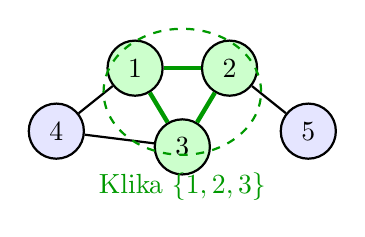
\begin{tikzpicture}[
  vnode/.style={circle, draw, minimum size=7mm, inner sep=0pt, fill=blue!10},
  thick
]
  \node[vnode, fill=green!20] (1) at (0, 1) {1};
  \node[vnode, fill=green!20] (2) at (1.2, 1) {2};
  \node[vnode, fill=green!20] (3) at (0.6, 0) {3};
  \node[vnode] (4) at (-1, 0.2) {4};
  \node[vnode] (5) at (2.2, 0.2) {5};
  
  \draw[green!60!black, ultra thick] (1) -- (2);
  \draw[green!60!black, ultra thick] (2) -- (3);
  \draw[green!60!black, ultra thick] (3) -- (1);
  
  \draw (1) -- (4);
  \draw (3) -- (4);
  \draw (2) -- (5);
  
  \draw[green!60!black, dashed] (0.6, 0.7) circle [x radius=1.0, y radius=0.8];
  \node[green!60!black] at (0.6, -0.5) {Klika $\{1,2,3\}$};
\end{tikzpicture}
\par\medskip
\textit{Obrázek 5.2: Graf obsahující kliku velikosti 3 (zvýrazněná zeleně).}
\end{center}